\chapter{A Brain-Inspired Algorithm}
\label{chp_htm}
\textit{Hierarchical Temporal Memory} (HTM) is a theory of how the human neocortex processes information, be it auditory, visual, motor, or somatosensory signals, developed by Jeff Hawkins \cite{Hawkins:2004:INT:993636}. It was long known that the neocortex looked remarkably similar in all different regions, this made anatomists to focus on the minuscule differences between the cortical regions to find the answer how they worked. However, in 1978, a neuroscientist by the name of Vernon B. Mountcaslte stopped focusing on the differences and saw that it was the similarities of the cortical regions that mattered. He came up with a theory of a single algorithm by which the neocortex processes information. The small differences that the anatomists found, was only because of the different types of signals that where being processed, not a difference in the algorithm itself \cite{Hawkins:2004:INT:993636}. With this idea of a single algorithm, Jeff Hawkins started a company called Numenta, with the intention of figuring out this algorithm. Numenta has since published an open-source project named Numenta Platform for Intelligent Computing, or NuPIC, which is an implementation of the HTM theory. 

In this chapter, we will start by introducing the HTM neuron. Then, we proceed to explain the way information is represented in an HTM network. Finally, we explain the sequence learning algorithm, called temporal memory.


\section{HTM Neuron Model}
The HTM neuron model is an abstraction of the pyramidal neuron in the neocortex \cite{10.3389/fncir.2016.00023}. However, so is the point neuron, which is used in most \textit{Artificial Neural Networks} (ANNs); so how different are they? The point neuron, see \autoref{fig:pointNeuron}, summates all the inputs on its synapses, then passes this value through a non-linear activation function. If the output value is above a threshold, the neuron outputs the value of the activation function; otherwise it will output a zero. With the properties of the dendrites explained in \autoref{sec:dendrite}, one could argue that point neurons does not have dendrites at all, and therefore completely lack the active properties of the dendrites. 


The connection between the point neurons is instead the synaptic connection, which can be changed via back propagation \cite{LeCunYann2015Dl}. 

\begin{figure}[ht!]
    \centering
    \input{background/HTM/tikz/pointNeuron.tex}
    \caption{The point neuron, used in most ANNs, summates the synaptic input and passes in through an activation function. It lacks active dendrites and only has synaptic connections.} %\cite{ANtikz}
    \label{fig:pointNeuron}
\end{figure}


The HTM neuron, see \autoref{fig:HTMNeuron}, is modelled on the active dendrite properties, and is therefore able to make use of the coincidence detection of the pyramidal neuron. The coincidence detection is activated via non-linear integration when a small number of synapses, experimentally show to be around 8-20, are active in close spatial proximity on a dendritic segment \cite{10.3389/fncir.2016.00023}. This non-linear integration will cause an NMDA dendritic spike, thus allowing the neuron to recognise a pattern \cite{10.3389/fncir.2016.00023}. In order for the neuron to be able to recognise a vast number of different patterns, the active input pattern needs to be sparse, i.e. only a few neurons that are active per input pattern. If we assume that the total number of neurons in a population is $n$, and at any given time the number of active cells are $a$, then sparse activation is given as $a \ll n$. On each dendritic segment there are $s$ number of synapses. For a dendritic segment to release an NMDA spike, the number of synapses that needs to be active is $\theta$, i.e. the NMDA spike threshold, of the total number of synapses $s$ \cite{10.3389/fncir.2016.00023}. By forming more synaptic connections for each pattern than necessary the neuron becomes more robust to noise and variation in the input pattern. However, the trade-off in these extra connections is the increased likelihood of the neuron to classify false positives, but if the patterns are sparse the increased likelihood is infinitesimal \cite{10.3389/fncir.2016.00023}. The dendrites can be divided into three zones of synaptic integration, the \textit{basal}, \textit{proximal}, and \textit{distal zone} \cite{10.3389/fncir.2016.00023}. These zones are categorised based on input and spatial position on the neuron, and are explained below.

\begin{figure}[ht!]
    \centering
    \hbox{\hspace{3.5em}\def\stepSym#1{
\begin{scope}[shift={#1}, scale=0.3]
    \coordinate (Aa) at (0,0) {};
    \coordinate (Bba) at (2.22,0) {};
    \coordinate (Bb) at (2,0) {};
    \coordinate (Cc) at (2,2) {};
    \coordinate (Ccd) at (1.78,2) {};
    \coordinate (Dd) at (4,2) {};

    \draw (Aa) -- (Bba);
    \draw(Bb) -- (Cc);
    \draw (Ccd) -- (Dd);
    \draw[thick] (2,1) circle (4cm);
\end{scope}
}


\def\slopeSym#1{
\begin{scope}[shift={#1}, scale=0.3]
    \coordinate (Aaa) at (0,0) {};
    \coordinate (Bbb) at (3,3) {};

    \draw (Aaa) -- (Bbb);
    \draw[thick] (1.5,1.5) circle (4cm);
\end{scope}
}


\begin{tikzpicture}[thick,scale=0.15, every node/.style={scale=.9}
    init/.style={
      draw,
      circle,
      inner sep=2pt,
      font=\Huge,
      join = by -latex
    },
    squa/.style={
      draw,
      inner sep=2pt,
      font=\Large,
      join = by -latex
    },
    start chain=2,node distance=13mm
    ]



%==============================
%PYRAMID
%==============================

\coordinate (A) at (-5,0) {};
\coordinate (B) at ( 5,0) {};
\coordinate (C) at (0,7) {};
\coordinate (D) at (0,35) {};
\coordinate (E) at (2.5,3.5) {};

\filldraw[draw=gray, thick,fill=gray!50] (A) -- (B) -- (C) -- cycle ;
\draw (A) -- (C);
\draw(B) -- (C);
\draw (A) -- (B);

%OR GATES
\node[or gate US, draw, rotate=180,logic gate inputs=nnnnn, scale=.6] at (15, 35) (or1) {};

\node[or gate US, draw, rotate=180,logic gate inputs=nnnnn, scale=.6] at (15, 13) (or2) {};

\stepSym{(25, 39)}

\stepSym{(25, 35)}

\stepSym{(25, 31)}




\stepSym{(25, 19)}

\stepSym{(25, 16)}

\stepSym{(25, 13)}

\stepSym{(25, 10)}

\stepSym{(25, 7)}

\slopeSym{(15,0)}

%INPUT
\draw (or1.output) -- (D);
\draw[-latex] (D) -- (C);

\draw[-latex] (or2.output) -- ([xshift=-1cm]or2.output) |- (E);



\draw (43, 0.4) -- node[below]{\tiny $\circ \circ  \bullet \circ \circ \circ \bullet \circ \circ \circ \circ \circ \bullet \bullet \circ$} (16.7, 0.4);
\draw[-latex] (14.2, 0.4) -- (10, 0.4) |- (3.5, 2.1);


\draw (26.8, 39.3) -- node[below]{\tiny $\bullet \circ \bullet \bullet \circ \circ \bullet \circ \bullet \circ \bullet$} (43, 39.3);
\draw (26.8, 35.3) -- node[below]{\tiny $\bullet \bullet \circ \circ \bullet \circ \bullet \bullet \circ \circ \bullet$} (43, 35.3);
\draw (26.8, 31.3) -- node[below]{\tiny  $\circ \bullet \circ \bullet \circ \bullet \circ \bullet \bullet \circ \bullet$} (43, 31.3);


\draw (26.8, 19.3) -- node[below]{\tiny $\bullet \bullet \circ \bullet \bullet \circ \bullet \bullet \bullet \circ \bullet$} (43, 19.3);
\draw (26.8, 16.3) -- node[below]{\tiny $\bullet \circ \bullet \bullet \bullet \circ \bullet \circ \bullet \bullet \bullet$} (43, 16.3);
\draw (26.8, 13.3) -- node[below]{\tiny $\bullet \bullet \circ \circ \bullet \circ \bullet \bullet \circ \circ \bullet$} (43, 13.3);
\draw (26.8, 10.3) -- node[below]{\tiny $\circ \bullet \bullet \bullet \circ \bullet \bullet \bullet \bullet \circ \bullet$} (43, 10.3);
\draw (26.8, 7.3) -- node[below]{\tiny  $\bullet \circ \circ \bullet \bullet \circ \bullet \bullet \circ \circ \bullet$} (43, 7.3);

\draw (24.4, 39.3) -- (or1);
\draw (24.4, 35.3) -- (or1);
\draw (24.4, 31.3) -- (or1);

\draw (24.4, 19.3) -- (or2);
\draw (24.4, 16.3) -- (or2);
\draw (24.4, 13.3) -- (or2);
\draw (24.4, 10.3) -- (or2);
\draw (24.4, 7.3) -- (or2);

%OUTPUT
\draw[-latex] (0,0) -- (0, -10);

\node[text width=3cm] (feedback) at (38,50)
    {Feedback};

\draw[-latex] (33.5, 48) -- (33.5, 41);

\node[text width=3cm] (context) at (62, 13.2)
    {Context};

\draw[-latex] (51, 13.2) -- (44, 13.2);

\node[text width=3cm] (feedforward) at (34, -10)
    {Feedforward};
    \draw[-latex] (30, -8) -- (30, -2);


\end{tikzpicture}}
    \caption{The schematic of the HTM neuron with arrays of coincident detectors consisting sets of synapses. However, in this figure only a few is shown, where black dots represents active synapses and white inactive ones. An NMDA spike is generated if the total number of active synapses are above the NMDA spike threshold, $\theta$, (represented as a Heaviside node) on any of the coincident detectors in a dendritic zone, which is represented by OR-gate. The dendritic zones can be divided in to three different zones base on the distance from the soma and synaptic connections. The proximal dendrites receive the \textit{feedforward} pattern, also know as the receptive field of the neuron. The basal zone receives information about the activity of neighbouring neurons of which its connected to and can be seen as giving \textit{context} to the input pattern. Apical dendrites receive the \textit{feedback} information form the layers above which also can effect the state of the soma \cite{10.3389/fncir.2016.00023}.}
    \label{fig:HTMNeuron}
\end{figure}



\subsection{Proximal Zone}
The feedforward input is received by the dendrites in the proximal zone, as this is the main receptive field of HTM neuron \cite{10.3389/fncir.2016.00023}. The proximal zone is the dendritic zone closest to the soma, usually consisting of several hundreds of synapses. Because of the proximity to the soma, the NMDA spike generated in this dendritic zone is strong enough to effect the soma in such a way that it generates an action potential. If the input pattern is sparse, subsets of synapses are able to generate NMDA spikes. Therefore, the coincident detector can detect multiple different feedforward patterns in one input signal, thus it can be viewed as a union of several unique patterns \cite{10.3389/fncir.2016.00023}.


\subsection{Basal Zone}
The basal zone is the dendritic segment that connects neuron in different minicolumns to each other. These connection allow a neuron to detect activity of neighbouring neurons, which enables individual neurons to learn transitions of input patterns. When a basal segment recognises a pattern, it will generate an NMDA spike. But due to the distance from the soma, the signal attenuates and is not able to generate an action potential in the soma. However, it does depolarise the soma, also called the \textit{predictive state} of the neuron. The \textit{predictive state} is an important state of the neuron because it has major contribution to the overall network functionality. If a neuron is in the predictive state it will become active earlier than its neighbours, in the same minicolumn and close proximity, if the feedforward pattern activates the proximal segment. When a neuron transitions from the predictive state to the active state it will not only give of an action potential, but also inhibit its neighbours from becoming active. Thus, keeping the activation pattern for recognised input patterns sparse \cite{10.3389/fncir.2016.00023}. This type of inhibition of nearby neurons is a way to represent the functionality of inhibition neurons, without representing them as individual cells \cite{10.3389/fncir.2017.00081}.


\subsection{Distal Zone}
Furthest from the soma is the apical dendrites, which connects neurons to the ascending layers. Much like the basal dendrites, apical segment does not generate a signal strong enough to cause an action potential in the soma. The signal generated on the apical segment differs from the signal generated on the basal segment. When a pattern is recognised, the NMDA spike does not directly travel to the soma. Instead, the soma is depolarises by a calcium ion, Ca$^{2+}$, spike generated at the dendritic segment. This depolarisation gives the neuron a ability of doing top-down extraction \cite{10.3389/fncir.2016.00023}.


\subsection{Learning}
The learning of an individual HTM neuron is based on two principles; formation and removal of synaptic connection via Hebbian style learning \cite{10.3389/fncir.2016.00023}. Each dendritic branch has a set of potential synaptic connection, where each connection can become active if there is enough simultaneous activity between the two potentially connected neurons. For a dendritic branch to recognise a pattern there needs to be a subset of the connected synapses that are active. This threshold is usually set to 15-20 \cite{10.3389/fncir.2016.00023}. When a dendritic branch becomes active, the entire dendritic segment is seen as active to the neuron, which is visualised in \autoref{fig:HTMNeuron} by the OR gate. The HTM neuron learns to detect new pattern by forming new synaptic connection on a dendritic branch. Each potential synaptic connection is given a \textit{permanence} value, which determines the strength of a synaptic connection between the neuron's dendritic branch and another neuron's axon in the network. The permanence value is defined on the range $[0, 1]$, where $0.0$ means that there is no connection, and $1.0$ means that a fully formed synapses has been grown. The potentiation and depression of each permanence value is achieved via a Hebbian learning rule, i.e. if neurons fire together they wire together. In order for a synaptic connection to be formed, the permanence value has to be above a certain threshold, e.g. $0.3$. With a permanence value above the threshold, the synaptic weight is assigned to 1 between the neurons. Therefore, there is no difference if the permanence value is $0.3$ or $1.0$ when a pattern is recognised. However, the lower the value is, the easier it is for the neuron to forget the connection, and in extension the pattern. With this growing mechanism of the neuron, the tolerance to noise and on-line learning is possible \cite{10.3389/fncir.2016.00023}. 





\section{Information Representation and Detection}
\subsection{Sparse Distributed Representation}
The presynaptic input patterns of information that is received by the dendrites, needs to be robust to noise and have a vast encoding capacity, as the neocortex handles an endless stream of sensory input. Empirical evidence shows that the neocortex operates by using sparse representations of information \cite{DBLP:journals/corr/AhmadH16}. In HTM theory, these sparse activation patterns are called \textit{Sparse Distributed Representation}, or SDR. Sparseness is due to the low number of active neurons at any given time, and it is distributed as no information is encoded in a single neuron. The information of the cell activity that the dendrite receives from the presynaptic cells is either active or non-active, and can therefore be modelled as a binary vector \cite{DBLP:journals/corr/AhmadH16}. 


\begin{figure}[ht!]
    \centering
    \resizebox{\textwidth}{!}{\centering
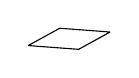
\begin{tikzpicture}
%\draw[help lines] (0,0) grid (10,10); %used just for visualising the positions of objects during construction


\begin{scope}[yshift=-180,yslant=.55,xslant=-1.6,scale=0.4]
        \ColorCells
        \draw (0, 0) grid (\GridSize, \GridSize);
        \coordinate (input);
\end{scope}

\end{tikzpicture}}
    \caption{An example of an SDR, where black squares represent active cells and white squares represent inactive ones. The SDR is represented as matrix for convenience.}
    \label{fig:sdr_ex}
\end{figure}


In \autoref{fig:sdr_ex}, we present an example of presynaptic input, or SDR, represented as a bit vector. Each cell can either be active or inactive, represented as black and white squares respectivly. The entire presynaptic input space of $n$ cells, at time $t$, for a dendritic segment is represented by an $n$-dimensional SDR, $\boldsymbol{X}_t$:


\begin{equation}
    \boldsymbol{X}_t = [b_0,\ b_1,...,\ b_{n-1}]
\end{equation}


\noindent where $b_i \in \mathbb{Z}_2$. The number of active cells is given by $w_X = | \boldsymbol{X}_t |$ and the pattern is considered sparse if $w_X \ll n$. The number of possible encodings the presynaptic input pattern is given by:


\begin{equation}
    \begin{pmatrix} n \\ w_X \end{pmatrix} = \frac{n!}{w_X!(n-w_X)!}
\end{equation}


\subsection{Presynaptic Pattern Detection}
A dendritic segment can also be modelled as a binary vector $\boldsymbol{D}$ of length $n$, which represents both potential and established synaptic connections to the presynaptic input. The active synaptic connections are represented as the non-zero elements, where $b_i$ is the synaptic connection to the presynaptic cell $i$. The number of established connections, represented by $s = | \boldsymbol{D} |$, has been experimentally shown to typically be around 20 to 300 synapses for a dendritic segment. But the potential connections can be in the thousands \cite{DBLP:journals/corr/AhmadH16}. To generate a spike in a dendritic segment, the number of synaptic connections that receive active input form the presynaptic cells needs to exceed a threshold, $\theta$. This threshold can be computed via the dot product of the two binary vectors:

\begin{equation}
    m(\boldsymbol{X}_t,\boldsymbol{D}) \equiv \boldsymbol{X}_t \cdot \boldsymbol{D} \geq \theta
\end{equation}


Where the threshold usually is lower than the number of connections and presynaptic activity, i.e. $\theta \leq s$ and $\theta \leq w_X$. As $\boldsymbol{X}_t$ does not represent the full presynaptic input pattern, but only a subsample, each dendritic segment only learns synaptic connections to some active cells of the entire pattern. How well a dendritic segment detects a pattern is dependent on the value of the NMDA spike threshold, $\theta$, and the robustness to noise in SDR encodings. With lower values of $\theta$ the dendritic branch is able to detect known input patterns easier. However, there is an inherent trade-off in small values of $\theta$, as the dendritic branch are then more likely to detect false positives if there is noise in the input pattern \cite{DBLP:journals/corr/AhmadH16}. 

If $\theta$ is set to a reasonable value, e.g. around 8-20, the probability of false detection due to noise in the SDR will be extremely unlikely. The reason for this is the sheer size of possible combination of ON-bits in the SDR. SDRs corrupted by some noise will not overlap enough to been interpreted as another possible input pattern. Therefore, detection on each dendritic segment with inexact matching has a very low probability of false detection, as described by Ahmad et al. in \cite{DBLP:journals/corr/AhmadH16}.


In each cortical region there are millions of neurons that simultaneously trying to recognise hundreds of patterns. They are able to recognise hundreds of patterns, as there only needs to be between 8 to 20 active synapses to generate an NMDA spike. On each of these neurons there are numerous dendritic branches, that combined have several thousands of synapses on them. Therefore, the robustness of the single dendritic segment needs to be maintained throughout a large neuron network \cite{DBLP:journals/corr/AhmadH16}. 


To quantify the robustness properties in the a larger scale we will first introduce the probability of false positives for an arbitrary number of dendritic segments, of which do not have to belong to the same neuron. Let $M$ be the number of different patterns represented by $M$ different dendritic segments, all of which has the threshold $\theta$ and $s$ number of synapses. The set of the dendritic segments is given by $S = \{ \boldsymbol{D}_0,\ \boldsymbol{D}_1,\ ...,\ \boldsymbol{D}_{M-1}  \}$, where $\boldsymbol{D}_i$ represents a dendritic segment vector. Let $\boldsymbol{X}_t$ be a random presynaptic input, of which is classified as belonging to the set if the following is true:


\begin{equation}
    \boldsymbol{X}_t \in S\ :=\ \exists_{\boldsymbol{D}_i}\ m(\boldsymbol{D}_i, \boldsymbol{X}_t) = True
\end{equation}


There is no false negatives if the number of corrupt bits in $\boldsymbol{X}_t$ is $\leq w_{D_i} - \theta$. The probability of a false positive is given by:

\begin{equation}
    P(\boldsymbol{X}_t \in S) = 1 - (1-P(m(\boldsymbol{X}_t, \boldsymbol{D}_i)))^M
\end{equation}

Which computationally difficult to compute as the probability of individual overlap is extremely unlikely \cite{DBLP:journals/corr/AhmadH16}.

\subsection{The Union Property on Dendritic Segments}
Another important property that comes with the SDR encoding is the ability to group and reliably store a set of SDR with a single SDR representation. This is achieved by taking the union of all the SDRs in a set, and is called the \textit{union property} \cite{DBLP:journals/corr/AhmadH16}. For binary vectors this is equivalent to taking the Boolean OR between all vectors. The ability to store multiple patterns is an important feature of the dendritic segment. In dendritic segments the synapses that respond to different patterns are stored in the same SDR. Thus, multiple presynaptic patterns can cause an NMDA spike to be generated. For a dendritic segment, $\boldsymbol{D}$, to be able to detect an arbitrary number of $M$ synaptic SDRs, we simply take union of all individual synaptic connection vectors, $\boldsymbol{d}_i$:

\begin{equation}
    \boldsymbol{D} = \bigcup_{i=0}^{M-1} \boldsymbol{d}_{i}
\end{equation}


The patterns will be detected as long as $\theta$ number of synapses are active. By increasing the $M$, the number of patterns that a dendritic segment can detect increases, but so does the probability of false detection. Therefore, there is a limit to the amount of ON-bits a dendritic segment can have, before the detection of false positives becomes a problem \cite{DBLP:journals/corr/AhmadH15}. Using unions, we are able to make temporal predictions, temporal pooling, create invariant representations, and create an effective hierarchy \cite{DBLP:journals/corr/AhmadH15}.








\begin{comment}
To prove the robustness to high levels of noise of the SDR encoding, $\boldsymbol{X}$, of $n$ presynaptic cells, we first need to explain the notion of \textit{overlap sets} and then \textit{inexact matching} \cite{DBLP:journals/corr/AhmadH16}. The overlap set allows us to examine the set of vectors of size $n$, that has $a$ ON-bits of which $b$ ON-bits overlap with $\boldsymbol{X}$. The number of vectors that belong to this set is defined as $\Omega_{\boldsymbol{X}}(n,a,b)$. Under the condition that $b \leq |\boldsymbol{X}|$ and $b \leq a$ we can compute the cardinality of this subset of vectors by: 

\begin{equation}
    |\Omega_X(n,a,b)| = \begin{pmatrix} |\boldsymbol{X}| \\ b \end{pmatrix} \times \begin{pmatrix} n - |\boldsymbol{X}| \\ a - b \end{pmatrix}
\end{equation}

\noindent Where the first term represents the number possible subsets of $\boldsymbol{X}$ that share $b$ on-bits, and the second term is all the patterns with $n - |\boldsymbol{X}|$ bits, of which the number of on-bits are $a - b$. Inexact matching allows us to give the probability that a dendritic segment, $\boldsymbol{D}$, will detect a random presynaptic activation pattern, $\boldsymbol{X}_t$  \cite{DBLP:journals/corr/AhmadH16}. The probability is given by the number of possible patterns that the dendritic segment can detect, divided by the number of possible activation patterns.

\begin{equation}
   P(m(\boldsymbol{X}_t, \boldsymbol{D}))  = \frac{\sum^{s}_{b=\theta}|\Omega_{\boldsymbol{D}}(n,w_X,b)|}{\begin{pmatrix} n \\ w_X \end{pmatrix}}
\end{equation}

This gives the probability of a false match for a given dendritic segment \cite{DBLP:journals/corr/AhmadH16}. If the presynaptic input pattern, $\boldsymbol{X}_t$, is corrupted by noise such that $v$ of the on-bits are now off, represented as $\boldsymbol{X}^{\prime}_t$, there is a probability of false negatives. The probability of a false negative increases with $v$, such that $\boldsymbol{X}^{\prime}_t \cdot \boldsymbol{D} < \theta$. As the overlap has to go below the threshold, there is no possibility of a false match if $v$ is sufficiently small, i.e. $v \leq s - \theta$. The computation of the probability of a false negative computed in a similar fashion to false positives \cite{DBLP:journals/corr/AhmadH16}. But instead of we have the cardinality of overlap set of $\boldsymbol{X}^{\prime}_t$ with respect to $\boldsymbol{D}$ in the numerator:

\begin{equation}
    |\Omega_{\boldsymbol{D}}(w_{X^{\prime}},v,b)| = \begin{pmatrix} s \\ b \end{pmatrix} \times \begin{pmatrix} w_{X^{\prime}} - s \\ v - b \end{pmatrix}
\end{equation}

\noindent And thus the probability of a false negative is given by:

\begin{equation}
   P(\boldsymbol{X}^{\prime}_t \cdot \boldsymbol{D} < \theta)  = \frac{\sum^{s}_{b=s - \theta + 1}|\Omega_{\boldsymbol{D}}(w_{X^{\prime}}, v, b)|}{\begin{pmatrix} w_{X^{\prime}} \\ v \end{pmatrix}}
\end{equation}

\end{comment}


\section{Temporal Memory}
\label{sec:TM}
\subsection{Notation}
The sequence learning algorithm of the HTM theory is called the \textit{temporal memory} \cite{10.3389/fncir.2016.00023}. The temporal memory consists of a layer of $N$ mini-columns stacked vertically. Each mini-column contains $M$ number of HTM neurons, thus a total of $NM$ cells. The cells can be in one of three states; active, non-active, or predictive (depolarised). Thus, for a given time-step, $t$, the active cells in the layer are represented by the $M \times N$ binary matrix, $\boldsymbol{A}^{t}$, where $a^{t}_{ij}$ is the current active (non-active) state of the $i$'th cell in the $j$'th minicolumn \cite{10.3389/fncir.2016.00023}. For the same time-step, the predictive state of each cell is given by the $M \times N$ binary matrix, $\boldsymbol{\prod}^{t}$, of which the predictive state of the $i$'th cell in $j$'th minicolumn is denoted by $\pi^{t}_{ij}$ \cite{10.3389/fncir.2016.00023}.


Each cell in a layer has the potential to connect to any other cell via its basal dendrites. The set of basal dendritic segments of the $i$'th cell in $j$'th minicolumn is therefore represented by $\boldsymbol{D}_{ij}$. Each segment has a subset of $s$ potential synaptic connections from the $NM - 1$ cells in the layer. This subset is associated with a non-zero permanence value, where the $d$'th dendritic segment is represented as a $M \times N$ sparse matrix, $\boldsymbol{D}^{d}_{ij}$. A synaptic connection is only considered to be established if the permanence value is above a certain threshold. To represent these synapses with a weight of 1 on the same dendritic segment, we have the following $M \times N$ binary matrix, $\tilde{\boldsymbol{D}}^{d}_{ij}$ \cite{10.3389/fncir.2016.00023}.

\subsection{Initialisation of the Dendritic Segments}
With the initialisation of the network, each cell's dendritic segments are randomly assigned unique sets of $s$ potential synaptic connections. The non-zero permanence value of these connections is randomly initialised, with some being above the threshold and thus being connected, while others are not and therefore are unconnected \cite{10.3389/fncir.2016.00023}.

\subsection{Activation of Cells}
Each minicolumns feedforward receptive field is a subset of the entire feedforward pattern \cite{10.3389/fncir.2016.00023}. The receptive field of a minicolumn is shared by all cells in that minicolumn. A minicolumn becomes active if the number of synapses connected to the receptive field is above a certain threshold. However, there is an upper bound of $k$ minicolumns that can be active at the same time. Thus the minicolumns that have the highest number of active synapses get selected, which is also called the inhibitory process \cite{10.3389/fncir.2016.00023}. The set of $k$ winning minicolumns is denoted by $\boldsymbol{W}^{t}$. The active state of the individual cells in each minicolumn is computed by:


\begin{equation}
    a_{ij}^{t} =
    \begin{cases}
      1,&\text{if } j \in \boldsymbol{W}^{t} \text{ and } \pi^{t-1}_{ij} = 1\\
      1,&\text{if } j \in \boldsymbol{W}^{t} \text{ and } \sum_i\pi^{t-1}_{ij} = 0\\
      0,&\text{otherwise}
    \end{cases}
\end{equation}


In the first case the cell will become active if it was in a predictive state in the time-step before. In the second case, all cells in a minicolumn will become active if none of them previously where in a predictive state. If none of these cases applies, the cell will remain inactive \cite{10.3389/fncir.2016.00023}. Next, the predictive state of each cell in the winning column is computed as follows:


\begin{equation}
    \pi^{t}_{ij} = 
        \begin{cases}
            1,&\text{if } \exists_d\ \Big\| \tilde{\boldsymbol{D}}^{d}_{ij} \circ \boldsymbol{A}^{t} \Big\|_1 > \theta\\
            0,&\text{otherwise}
        \end{cases}
\end{equation}


For a cell to become depolarised in the current time-step, the contextual information received from the presynaptic input on any basal dendritic segment needs to be above the NMDA spike threshold, $\theta$. In order to detect if a segment is above this threshold, an element-wise multiplication, represented by $\circ$, of the dendritic segment and the active cells in the layer is computed. The $L_1$-norm of the result is then computed and compared with the threshold. In order for a cell to become depolarise, at least one segment needs to be active \cite{10.3389/fncir.2016.00023}.
 
\subsection{Learning of Dendritic Segments}
The reason a layer is able to learn multiple functionalities is due to the plasticity of the synapses belonging the cells \cite{10.3389/fncir.2016.00023}. In the HTM neuron, the updating rule for the permanence value of the synapses is a Hebbian-like rule. That is, if a cell was in a predictive state in a previous time-step, and then becomes active in the current because of the feedforward pattern, the synaptic connection that cause the depolarisation gets reinforced \cite{10.3389/fncir.2016.00023}. The segments responsible for the depolarisation are selected via the following operation:


\begin{equation}
    \label{eq:tm_predicted}
    \forall_{j\in\boldsymbol{W}^{t}}\ \Big( \pi^{t-1}_{ij} > 0 \Big) \text{ and } \Big\| \tilde{\boldsymbol{D}}^{d}_{ij} \circ \boldsymbol{A}^{t-1} \Big\|_1 > \theta
\end{equation}


First, the winning columns that had cells in a predictive state is selected. Next, the dendritic segments of these cells that cause the depolarisation is selected. However, if a winning column did not have cells in a predicted state, we need to reinforce the connection of the cell that had the most active segment. As this allows the cell to represent the transition of the sequence if it repeats later on \cite{10.3389/fncir.2016.00023}. To select the segment that where the most active, we first denote $\dot{\boldsymbol{D}^{d}_{ij}}$ as the $M \times N$ binary matrix of $\boldsymbol{D}^{d}_{ij}$, where each positive permanence value is represented as a 1 \cite{10.3389/fncir.2016.00023}. Next, we select the winning columns that did not have a cell in a predictive state, and then take the cell with the most active dendritic segment in each minicolumn.

\begin{equation}
    \label{eq:tm_close}
    \forall_{j\in\boldsymbol{W}^{t}}\ \Big( \sum_{i}\pi^{t-1}_{ij} = 0 \Big) \text{ and } \Big\| \tilde{\boldsymbol{D}}^{d}_{ij} \circ \boldsymbol{A}^{t-1} \Big\|_1 = max_i\Big(\Big\| \dot{\boldsymbol{D}}^{d}_{ij} \circ \boldsymbol{A}^{t-1} \Big\|_1 \Big)
\end{equation}


With the ability to select the relevant segments that cause a cell to become active, we now need to define the Hebbian-like learning rule, i.e. wire together fire together. That is, we reward connections with active presynaptic input, and punish the synapses that does not. To achieve this we decrease all permanence values by a small value $p^-$, while at the same time rewarding the connection with active presynaptic input by increasing them with a larger value $p^+$ \cite{10.3389/fncir.2016.00023}. 

\begin{equation}
    \label{eq:update_tm}
    \Delta \boldsymbol{D}^{d}_{ij} = p^+\Big(\dot{\boldsymbol{D}}^{d}_{ij} \circ \boldsymbol{A}^{t}\Big) - p^-\dot{\boldsymbol{D}}^{d}_{ij}
\end{equation}


As \autoref{eq:update_tm} only updates cells that became active, or closest to being active, selected by  \autoref{eq:tm_predicted} and \autoref{eq:tm_close} respectively, we need to define an equation for penalising the cells that did not become active \cite{10.3389/fncir.2016.00023}. The permanence values of these inactive cells will start to decay with a small value of $p^{--}$:

\begin{equation}
        \Delta \boldsymbol{D}^{d}_{ij} = p^{--}\dot{\boldsymbol{D}}^{d}_{ij} \text{ where } a_{ij}^t = 0 \text{ and } \Big\| \tilde{\boldsymbol{D}}^{d}_{ij} \circ \boldsymbol{A}^{t} \Big\|_1 > \theta
\end{equation}

Each cell is then updated with new permanence values for each of its dendritic segments by applying the following update rule:

\begin{equation}
    \boldsymbol{D}^{d}_{ij} = \boldsymbol{D}^{d}_{ij} + \Delta \boldsymbol{D}^{d}_{ij}
\end{equation}


As we have now gone through the temporal learning algorithm, we will now summarise this chapter. First, we introduced the HTM neuron and how it is modelled differently from the point neuron used in most ANNs. We then explained the properties of each dendritic segment of the HTM neuron. Then, we moved on to explaining how an HTM neuron learns to recognise input patterns. Next, we introduced the notion of sparse distributed representations (SDRs), which are binary vectors that represent information in an HTM network. With the familiarity of SDRs, we then went over the active processing property of the dendritic segment, and how each segment can detect multiple input patterns, i.e. with the \textit{union property}. Finally, we went over the algorithm for recognising temporal sequences in an HTM network and how it is able to learn to recognise new input patterns. 











\begin{comment}

\begin{figure}[H]
    \centering
    \scalebox{.4}{\input{background/HTM/tikz/minicol.tex}}
    \caption{Caption}
    \label{fig:my_label}
\end{figure}

\begin{figure}[H]
    \centering
    \scalebox{.2}{\centering
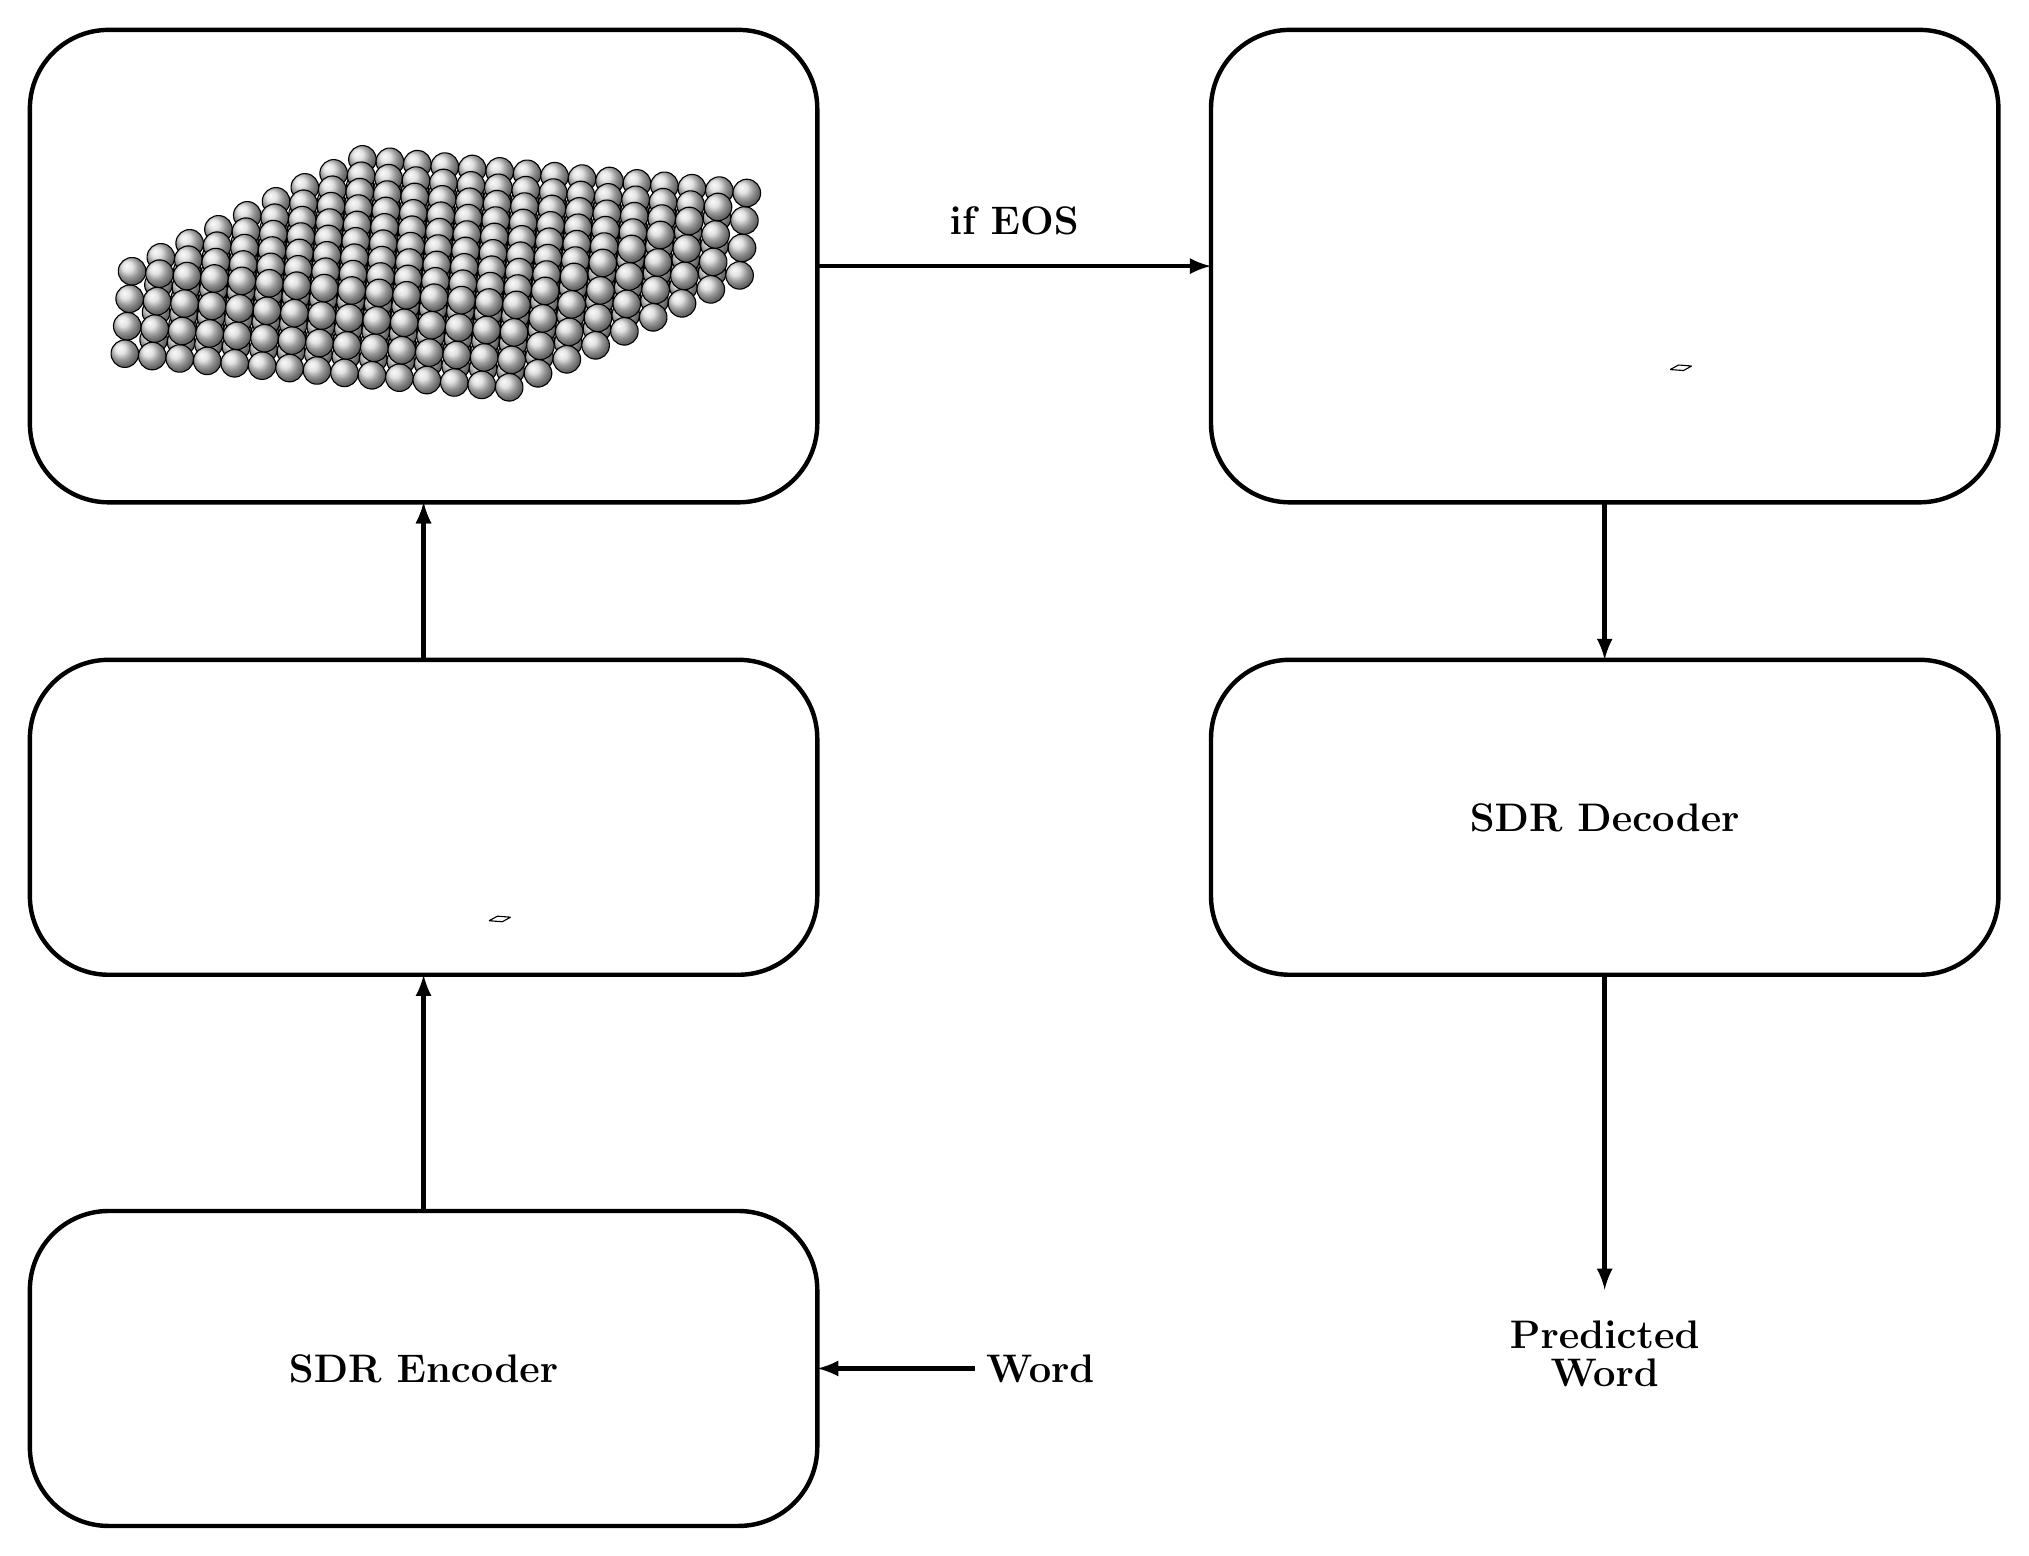
\begin{tikzpicture}



\draw[-latex,ultra thick] (6,-12) to node [right=1cm] {\Large\textbf{Word}} (4,-12);

\draw [rounded corners=1cm,ultra thick] (-6,-14) rectangle ++(10,4) node [midway] {\Large\textbf{SDR Encoder}};


\draw[-latex,ultra thick](-1,-10) to (-1,-7);



\draw [rounded corners=1cm,ultra thick] (-6,-7) rectangle ++(10,4) node [midway] {};
\begin{scope}[yshift=-180,yslant=.55,xslant=-1.6,scale=0.105]
        \ColorCells
        \draw (0, 0) grid (\GridSize, \GridSize);
        \coordinate (input);
\end{scope}

\draw[-latex,ultra thick](-1,-3) to (-1,-1);


\draw [rounded corners=1cm,ultra thick] (9,-1) rectangle ++(10,6) node [midway] {};
\begin{scope}[xshift=15cm, yshift=7cm, yshift=-180, yslant=.55, xslant=-1.6, scale=0.105] 
    \ColorCells
    \draw (0, 0) grid (\GridSize, \GridSize);
    \coordinate (output);
\end{scope}  


\draw[-latex,ultra thick](-1,-3) to (-1,-1);

\draw[-latex,ultra thick] (4,2) to node [above=.25cm] {\Large\textbf{if EOS}} (9,2);


\draw[-latex,ultra thick](14,-1) to (14,-3);

\draw [rounded corners=1cm,ultra thick] (9,-7) rectangle ++(10,4) node [midway] {\Large\textbf{SDR Decoder}};


\draw[-latex,ultra thick] (14,-7) to node [below=2.25cm] {\begin{tabular}{c} \Large\textbf{Predicted} \\ \Large\textbf{Word} \end{tabular}} (14,-11);


\draw [rounded corners=1cm,ultra thick] (-6,-1) rectangle ++(10,6) node [midway] {};

\begin{scope}[rotate around = {-5:(0,20,20)}, yshift=2.5cm,xshift=-0.5cm,scale=0.7]
   
    \foreach \x  in {0.75,1.25,1.75,2.25,2.75,3.25,3.75,4.25,4.75,5.25,5.75,6.25,6.75,7.25,7.75}%
        \shadedraw [ball color= gray!30] (\x,2,1.55*2.5) circle (0.25cm);
    \foreach \x  in {0.75,1.25,1.75,2.25,2.75,3.25,3.75,4.25,4.75,5.25,5.75,6.25,6.75,7.25,7.75}%
        \shadedraw [ball color= gray!30] (\x-.2,2,1.55*3) circle (0.25cm);
    \foreach \x  in {0.75,1.25,1.75,2.25,2.75,3.25,3.75,4.25,4.75,5.25,5.75,6.25,6.75,7.25,7.75}%
        \shadedraw [ball color= gray!30] (\x-.4,2,1.55*3.5) circle (0.25cm);
    \foreach \x  in {0.75,1.25,1.75,2.25,2.75,3.25,3.75,4.25,4.75,5.25,5.75,6.25,6.75,7.25,7.75}%
        \shadedraw [ball color= gray!30] (\x-.6,2,1.55*4) circle (0.25cm);
    \foreach \x  in {0.75,1.25,1.75,2.25,2.75,3.25,3.75,4.25,4.75,5.25,5.75,6.25,6.75,7.25,7.75}%
        \shadedraw [ball color= gray!30] (\x-.8,2,1.55*4.5) circle (0.25cm);
    \foreach \x  in {0.75,1.25,1.75,2.25,2.75,3.25,3.75,4.25,4.75,5.25,5.75,6.25,6.75,7.25,7.75}%
        \shadedraw [ball color= gray!30] (\x-1,2,1.55*5) circle (0.25cm);
    \foreach \x  in {0.75,1.25,1.75,2.25,2.75,3.25,3.75,4.25,4.75,5.25,5.75,6.25,6.75,7.25,7.75}%
        \shadedraw [ball color= gray!30] (\x-1.2,2,1.55*5.5) circle (0.25cm);
    \foreach \x  in {0.75,1.25,1.75,2.25,2.75,3.25,3.75,4.25,4.75,5.25,5.75,6.25,6.75,7.25,7.75}%
        \shadedraw [ball color= gray!30] (\x-1.4,2,1.55*6) circle (0.25cm);
    \foreach \x  in {0.75,1.25,1.75,2.25,2.75,3.25,3.75,4.25,4.75,5.25,5.75,6.25,6.75,7.25,7.75}%
        \shadedraw [ball color= gray!30] (\x-1.6,2,1.55*6.5) circle (0.25cm);


    \foreach \x  in {0.75,1.25,1.75,2.25,2.75,3.25,3.75,4.25,4.75,5.25,5.75,6.25,6.75,7.25,7.75}%
        \shadedraw [ball color= gray!30] (\x,2.5,1.55*2.5) circle (0.25cm);
    \foreach \x  in {0.75,1.25,1.75,2.25,2.75,3.25,3.75,4.25,4.75,5.25,5.75,6.25,6.75,7.25,7.75}%
        \shadedraw [ball color= gray!30] (\x-.2,2.5,1.55*3) circle (0.25cm);
    \foreach \x  in {0.75,1.25,1.75,2.25,2.75,3.25,3.75,4.25,4.75,5.25,5.75,6.25,6.75,7.25,7.75}%
        \shadedraw [ball color= gray!30] (\x-.4,2.5,1.55*3.5) circle (0.25cm);
    \foreach \x  in {0.75,1.25,1.75,2.25,2.75,3.25,3.75,4.25,4.75,5.25,5.75,6.25,6.75,7.25,7.75}%
        \shadedraw [ball color= gray!30] (\x-.6,2.5,1.55*4) circle (0.25cm);
    \foreach \x  in {0.75,1.25,1.75,2.25,2.75,3.25,3.75,4.25,4.75,5.25,5.75,6.25,6.75,7.25,7.75}%
        \shadedraw [ball color= gray!30] (\x-.8,2.5,1.55*4.5) circle (0.25cm);
    \foreach \x  in {0.75,1.25,1.75,2.25,2.75,3.25,3.75,4.25,4.75,5.25,5.75,6.25,6.75,7.25,7.75}%
        \shadedraw [ball color= gray!30] (\x-1,2.5,1.55*5) circle (0.25cm);
    \foreach \x  in {0.75,1.25,1.75,2.25,2.75,3.25,3.75,4.25,4.75,5.25,5.75,6.25,6.75,7.25,7.75}%
        \shadedraw [ball color= gray!30] (\x-1.2,2.5,1.55*5.5) circle (0.25cm);
    \foreach \x  in {0.75,1.25,1.75,2.25,2.75,3.25,3.75,4.25,4.75,5.25,5.75,6.25,6.75,7.25,7.75}%
        \shadedraw [ball color= gray!30] (\x-1.4,2.5,1.55*6) circle (0.25cm);
    \foreach \x  in {0.75,1.25,1.75,2.25,2.75,3.25,3.75,4.25,4.75,5.25,5.75,6.25,6.75,7.25,7.75}%
        \shadedraw [ball color= gray!30] (\x-1.6,2.5,1.55*6.5) circle (0.25cm);


    \foreach \x  in {0.75,1.25,1.75,2.25,2.75,3.25,3.75,4.25,4.75,5.25,5.75,6.25,6.75,7.25,7.75}%
        \shadedraw [ball color= gray!30] (\x,3,1.55*2.5) circle (0.25cm);
    \foreach \x  in {0.75,1.25,1.75,2.25,2.75,3.25,3.75,4.25,4.75,5.25,5.75,6.25,6.75,7.25,7.75}%
        \shadedraw [ball color= gray!30] (\x-.2,3,1.55*3) circle (0.25cm);
    \foreach \x  in {0.75,1.25,1.75,2.25,2.75,3.25,3.75,4.25,4.75,5.25,5.75,6.25,6.75,7.25,7.75}%
        \shadedraw [ball color= gray!30] (\x-.4,3,1.55*3.5) circle (0.25cm);
    \foreach \x  in {0.75,1.25,1.75,2.25,2.75,3.25,3.75,4.25,4.75,5.25,5.75,6.25,6.75,7.25,7.75}%
        \shadedraw [ball color= gray!30] (\x-.6,3,1.55*4) circle (0.25cm);
    \foreach \x  in {0.75,1.25,1.75,2.25,2.75,3.25,3.75,4.25,4.75,5.25,5.75,6.25,6.75,7.25,7.75}%
        \shadedraw [ball color= gray!30] (\x-.8,3,1.55*4.5) circle (0.25cm);
    \foreach \x  in {0.75,1.25,1.75,2.25,2.75,3.25,3.75,4.25,4.75,5.25,5.75,6.25,6.75,7.25,7.75}%
        \shadedraw [ball color= gray!30] (\x-1,3,1.55*5) circle (0.25cm);
     \foreach \x  in {0.75,1.25,1.75,2.25,2.75,3.25,3.75,4.25,4.75,5.25,5.75,6.25,6.75,7.25,7.75}%
        \shadedraw [ball color= gray!30] (\x-1.2,3,1.55*5.5) circle (0.25cm);
    \foreach \x  in {0.75,1.25,1.75,2.25,2.75,3.25,3.75,4.25,4.75,5.25,5.75,6.25,6.75,7.25,7.75}%
        \shadedraw [ball color= gray!30] (\x-1.4,3,1.55*6) circle (0.25cm);
    \foreach \x  in {0.75,1.25,1.75,2.25,2.75,3.25,3.75,4.25,4.75,5.25,5.75,6.25,6.75,7.25,7.75}%
        \shadedraw [ball color= gray!30] (\x-1.6,3,1.55*6.5) circle (0.25cm);
    
    
    
    \foreach \x  in {0.75,1.25,1.75,2.25,2.75,3.25,3.75,4.25,4.75,5.25,5.75,6.25,6.75,7.25,7.75}%
        \shadedraw [ball color= gray!30] (\x,3.5,1.55*2.5) circle (0.25cm);
    \foreach \x  in {0.75,1.25,1.75,2.25,2.75,3.25,3.75,4.25,4.75,5.25,5.75,6.25,6.75,7.25,7.75}%
        \shadedraw [ball color= gray!30] (\x-.2,3.5,1.55*3) circle (0.25cm);
    \foreach \x  in {0.75,1.25,1.75,2.25,2.75,3.25,3.75,4.25,4.75,5.25,5.75,6.25,6.75,7.25,7.75}%
        \shadedraw [ball color= gray!30] (\x-.4,3.5,1.55*3.5) circle (0.25cm);
    \foreach \x  in {0.75,1.25,1.75,2.25,2.75,3.25,3.75,4.25,4.75,5.25,5.75,6.25,6.75,7.25,7.75}%
        \shadedraw [ball color= gray!30] (\x-.6,3.5,1.55*4) circle (0.25cm);
    \foreach \x  in {0.75,1.25,1.75,2.25,2.75,3.25,3.75,4.25,4.75,5.25,5.75,6.25,6.75,7.25,7.75}%
        \shadedraw [ball color= gray!30] (\x-.8,3.5,1.55*4.5) circle (0.25cm);
    \foreach \x  in {0.75,1.25,1.75,2.25,2.75,3.25,3.75,4.25,4.75,5.25,5.75,6.25,6.75,7.25,7.75}%
        \shadedraw [ball color= gray!30] (\x-1,3.5,1.55*5) circle (0.25cm);
    \foreach \x  in {0.75,1.25,1.75,2.25,2.75,3.25,3.75,4.25,4.75,5.25,5.75,6.25,6.75,7.25,7.75}%
        \shadedraw [ball color= gray!30] (\x-1.2,3.5,1.55*5.5) circle (0.25cm);
    \foreach \x  in {0.75,1.25,1.75,2.25,2.75,3.25,3.75,4.25,4.75,5.25,5.75,6.25,6.75,7.25,7.75}%
        \shadedraw [ball color= gray!30] (\x-1.4,3.5,1.55*6) circle (0.25cm);
    \foreach \x  in {0.75,1.25,1.75,2.25,2.75,3.25,3.75,4.25,4.75,5.25,5.75,6.25,6.75,7.25,7.75}%
        \shadedraw [ball color= gray!30] (\x-1.6,3.5,1.55*6.5) circle (0.25cm); 
\end{scope}
\end{tikzpicture}}
    \caption{Caption}
    \label{fig:my_label}
\end{figure}
\end{comment}

